\documentclass{beamer}
\usepackage[utf8]{inputenc}

\usepackage{amsmath,amsfonts,amssymb,amsthm,
mathtools,mathrsfs}
\usepackage{physics}
\usepackage{xcolor}
\usepackage{listings}

\usetheme{Madrid}
\usecolortheme{default}
\useoutertheme[subsection=false]{miniframes}

\addtobeamertemplate{block example begin}{%
    \setlength{\textwidth}{0.8\textwidth}
}{}

\usepackage[style=apa, backend=biber, natbib]{biblatex}
\addbibresource{references.bib}


\title[ABM Workshop]{Agent-Based Simulations for Protocol Design, Tokenomics, and Risk Analysis}
\subtitle{ETHChicago 2023}
\author[Mingxuan He]{Mingxuan He\\
mingxuanh.eth}


\institute[]{
Phoenix graduate scholar (computational economics), University of Chicago\\
Research fellow, Nethermind
}


\date{\today}


% table of contents page before each section (optional)
% \AtBeginSection[]
% {
%   \begin{frame}
%     \frametitle{Table of Contents}
%     \tableofcontents[currentsection]
%   \end{frame}
% }


\begin{document}

% title page
\begin{frame}
    \titlepage
\end{frame}

% table of contents
\begin{frame}
    \frametitle{Agenda}
    \tableofcontents
\end{frame}


%----------------
\section{Introduction}
\begin{frame}{What are Agent-Based Models?}
    A programmed world where multiple \textbf{agents} live in an enviornment and interact with each other through \textbf{actions}.
    
    \begin{itemize}
        \item Agents can represent:
              \begin{itemize}
                  \item individuals (humans, wallets, network nodes)
                  \item organizations/abstract entities (DAOs, protocols)
              \end{itemize}
        \item Actions:
              \begin{itemize}
                  \item economic (send/receive, buy/sell, deposit/withdraw)
                  \item social (vote, follow/unfollow)
              \end{itemize}
    \end{itemize}
\end{frame}


\begin{frame}{What can you do with an ABM simulation?}

    \begin{itemize}
        \item For users / investors: \\
        Manage risk by stress-testing the protocol with hypothetical market events like hacks and price crashes.
              \bigskip
        \item For protocol / DApp engineers: \\
        Make design decisions (e.g. fee rates, reward tokenomics) by simulating all possibilities and optimize for the best outcome
    \end{itemize}
% ABMs are great for modeling Web3 protocols because of their decentralized nature -- individual-level behaviors are easy to observe from public wallet/contract data, and system rules are clear (written in smart contracts)
\end{frame}


\begin{frame}{Traditional Method vs ABM}
    \begin{columns}
        \column{0.5\textwidth}
        Macro-level simulation\\
        \begin{itemize}
            \item Only measures aggregate outcomes (net gains/losses)
            \item More assumptions required
            \item Fixed parameters
        \end{itemize}

        \column{0.5\textwidth}
        Agent-based simulation\\
        \begin{itemize}
            \item Measures individual-level \& aggregate outcomes
            \item Less assumptions required
            \item Customizable parameters
        \end{itemize}
    \end{columns}

    \bigskip\bigskip
    \textit{``All models are wrong, but some are useful."}

\end{frame}


%----------------
%\section{Tools}




% \begin{frame}{Data Sources}
%     To make the model realistic, we must draw observations from real-world data:
%     \begin{itemize}
%         \item Raw onchain data: \textit{Etherscan, AWS Public Blockchain Data}
%         \item Aggregated databases: \textit{Dune, Flipside, Footprint}
%         \item Analytics providers: \textit{Nansen, DeFiLlama, etc.}
%         \item Protocol reported dashboards/stats page
%         \item See \href{https://sites.google.com/view/mingxuanhe/resources}{\underline{sites.google.com/view/mingxuanhe/resources}}\\
%     \end{itemize}
%     \bigskip
%     Example use case:\\
%     Check \#N of wallets currently holding token X on Dune\\
%     $\rightarrow$ enter \#N as initial value for user agents
% \end{frame}


% \begin{frame}{Data Analysis Tools}
%     Some numbers cannot be directly observed, so we need some data analysis / modeling tools for estimating them. The standard is Python with packages like:
%     \begin{itemize}
%         \item Stats/ML: \textit{scipy, statsmodels, sklearn}
%         \item Visualization: \textit{matplotlib, seaborn, plotly}
%         \item Basic functionality: \textit{pandas, numpy}
%     \end{itemize}
%     Note: R/Matlab/Julia are good alternatives for this part alone, but do not work with Mesa.
% \end{frame}


%----------------
\section{Modeling Steps}

\begin{frame}{Step 0: Understand your protocol}
    Ask questions like:
    \begin{itemize}
        \item Who are the primary group of actors involved in the ecosystem?
        \item What can each actor do?
        \item What rules does the system set for agents?
        \item Is there any tokens involved and if so how do they flow?
    \end{itemize}
    \begin{block}{Excercise}
        Pick a protocol / DApp and try to answer these questions.
    \end{block}
\end{frame}

\begin{frame}{Step 1: Build a flow chart}
    A flow chart is the best way to start modeling complex systems like DeFi protocols. Be sure to include:
    \begin{itemize}
        \item Agent-agent interactions
        \item Agent-protocol interactions
        \item Flow of funds / native tokens
    \end{itemize}
    Recommended tool: Draw.io (open source)\\
    \begin{figure}
        \centering
        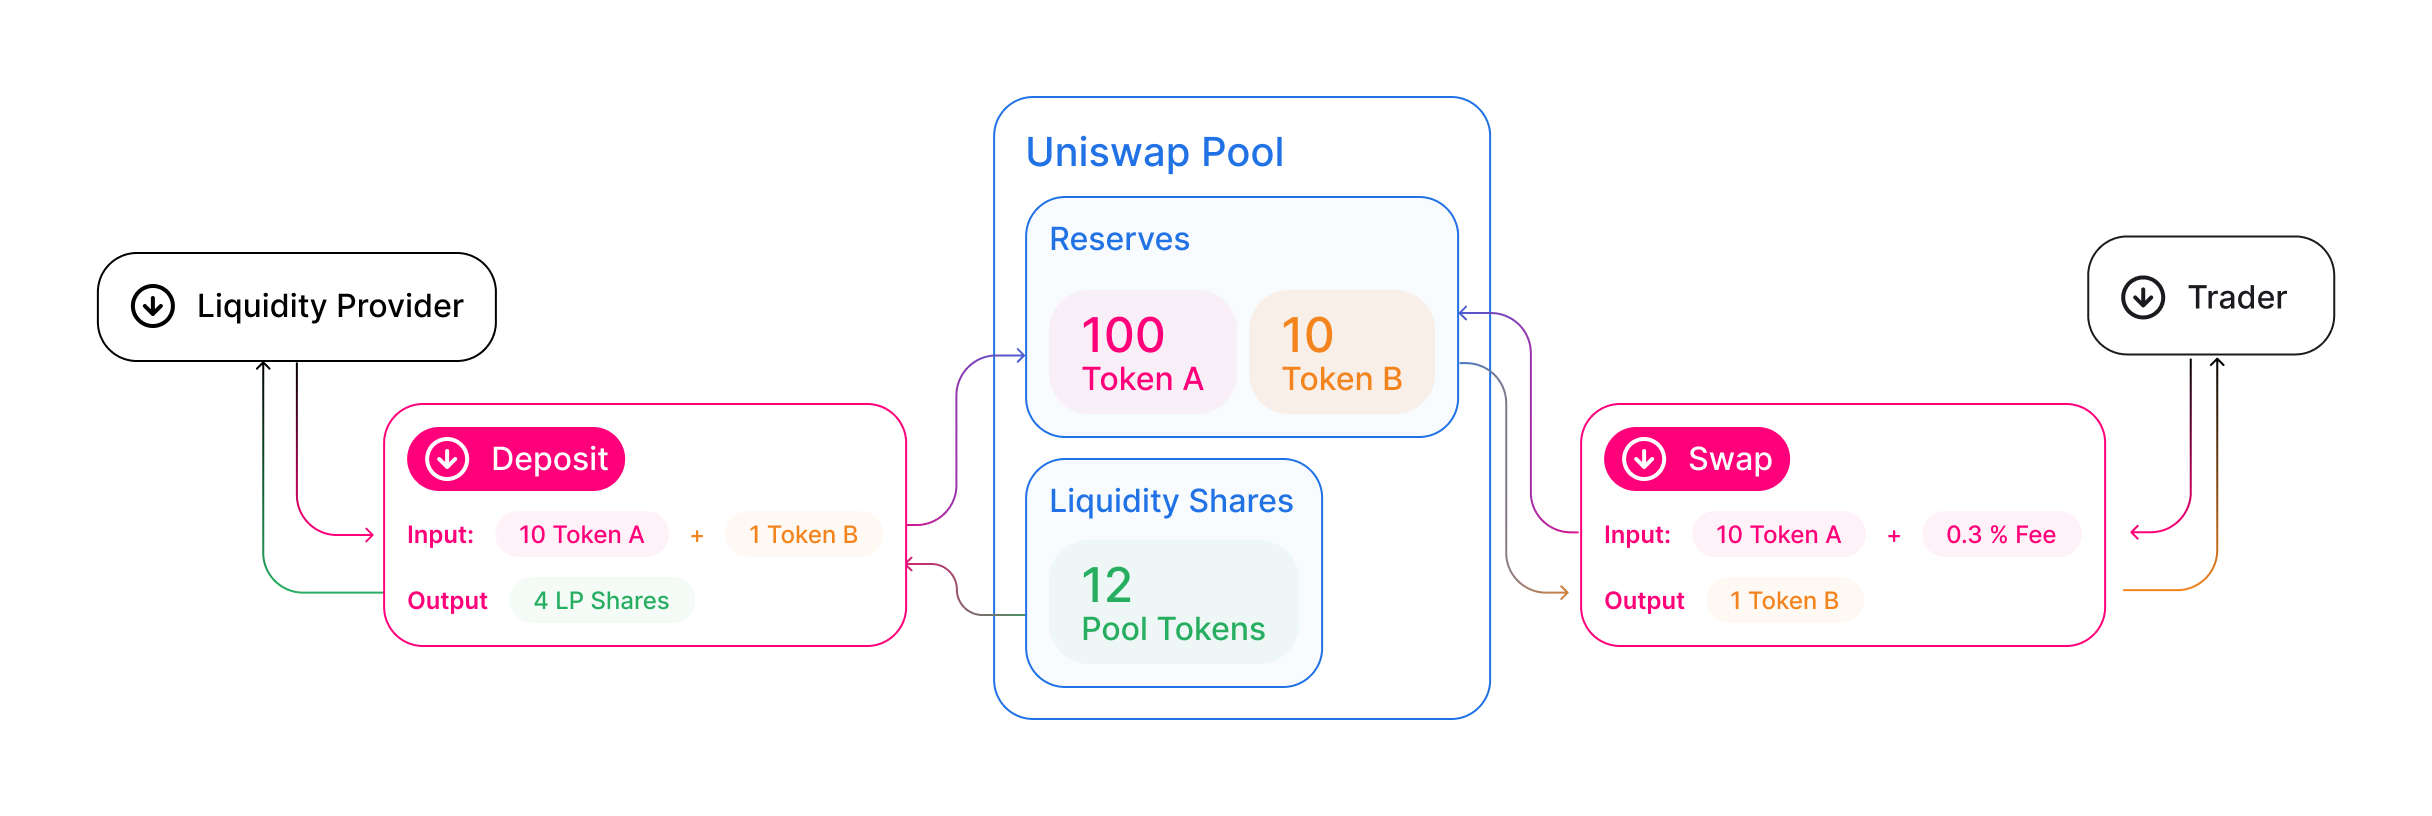
\includegraphics[width=\textwidth]{figures/uni_flowchart.jpg}
    \end{figure}
\end{frame}

\begin{frame}{Mesa}
    Open-source Python library for agent based models and simulations\\
    \begin{itemize}
        \item Easy to use (entry-level OOP knowledge)
        \item Built-in analysis and visualization modules
    \end{itemize}
    \begin{figure}
        \centering
        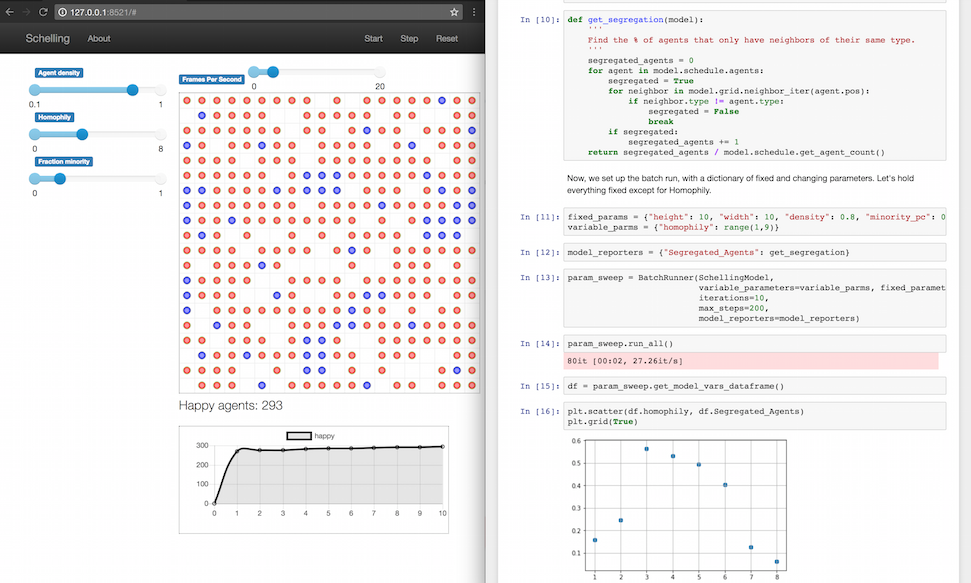
\includegraphics[width=0.8\textwidth]{figures/Mesa_Screenshot.png}
    \end{figure}
\end{frame}

\begin{frame}[fragile]{Step 2: Create agent classes}
    \begin{columns}
        \column{0.5\textwidth}
        \begin{block}{Code Structure}
            \begin{lstlisting}[language=Python, basicstyle=\footnotesize, xleftmargin=-16pt, columns=fullflexible]
    class TestAgent(mesa.Agent):
      
      def __init__(self, unique_id, model):
        super().__init__(unique_id, model)
        self.unique_id = unique_id
        self.model = model
        self.attr_X = 0
        self.attr_Y = 0
        
      def step(self):
        # observe state and perform actions
      
      def action_name(self, args):
        # single action function
    
    \end{lstlisting}
        \end{block}

        \column{0.5\textwidth}
        \begin{itemize}
            \item Subclass \textit{mesa.Agent}
            \item Define \textbf{attributes} and \textbf{actions}.
            \item Define a \textbf{step} (policy) function
        \end{itemize}
    \end{columns}

\end{frame}


\begin{frame}[fragile]{Step 3: Create model class}
    \begin{columns}
        \column{0.5\textwidth}

        \begin{block}{Code Structure}
            \begin{lstlisting}[language=Python, basicstyle=\footnotesize, xleftmargin=-16pt, columns=fullflexible]
    from mesa.time import RandomActivation
    
    class TestModel(mesa.Model):
      def __init__(self, params, seed=None):
        super().__init__()
        self.schedule = RandomActivation()
        for i in range(100):
          agnt = TestAgent(i, self)
          self.schedule.add(agnt)
        self.datacollector = mesa.DataCollector(
          agent_reporters={"x": "attr_X"})
        
      def step(self):
        self.add_remove_agents()
        self.schedule.step()
        self.datacollector.collect(self)
    \end{lstlisting}
        \end{block}

        \column{0.5\textwidth}
        \begin{itemize}
            \item Subclass \textit{mesa.Model}
            \item Create an initial state
            \item A mechanism to add / remove user agents each step
            \item Assign agents to a scheduler
            \item Create data collectors
        \end{itemize}

    \end{columns}

\end{frame}


\begin{frame}[fragile]{Step 4: Calibration and estimation}
    Aim: Assigning values to parameters and initial conditions in order to \underline{reproduce real-world behavior}.

    \bigskip
    
    Methods:
    \begin{itemize}
        \item Direct observation from data / protocol parameters\\
        e.g. 5\% inflation rate on token, 15\% node commission
        \item Statistical estimation (minimize distance from real data)\\
        e.g. monthly new users, daily ETH prices
        \item Meta-modeling
    \end{itemize}
    For a list of data sources and tools for on-chain analytics, see \href{https://sites.google.com/view/mingxuanhe/resources}{\underline{sites.google.com/view/mingxuanhe/resources}}
\end{frame}

\begin{frame}{Step 5: Simulation}
    Data tracking: \textit{mesa.DataCollector}\\
    Track both aggregate variables (e.g. TVL, total fees) and individual agent variables (e.g. distribution of token balance, top and bottom performance of agents)

    \bigskip
    
    Tips:
    \begin{itemize}
        \item Run multiple batches on different random seeds and aggregate (Monte Carlo)
        \item Change the protocol parameters to explore ``parallel universes"
        \item Disaster simulation: large drop in prices, large withdrawl of liquidity, etc.
    \end{itemize}
\end{frame}


\begin{frame}{Step 6: Visualization (optional)}
    Use \textit{mesa.visualization.modules}\\
    Available modules:
    \begin{itemize}
        \item Charts: bar chart, line chart, pie chart
        \item Grids: canvas grid, hex grid
        \item Network visualization
        \item User-settable parameter (slider / choice / number input)
    \end{itemize}


\end{frame}


\section{Demo}

\begin{frame}{Example: An ABM for Uniswap V2 AMM}
    \begin{itemize}
        \item Agents: 1000 traders, 50 liquidity providers, 1 liquidity pool for token pair X and Y
        \item Actions: traders can swap, LPs can add/remove liquidity
        \item Agent attributes:
              \begin{itemize}
                  \item Trader: holding of token X and Y
                  \item LP: holding of token X and Y, holding of LP tokens
                  \item Pool: balance of token X and Y, fee rate, constant product $K$
              \end{itemize}
              %\item Parameters: 
        \item Performance metrics: TVL, slippage, impermenant loss
    \end{itemize}
\end{frame}

\begin{frame}{Extensions to the Toy Model}
    \begin{itemize}
        \item Different types of traders: arbitrageurs, speculators, noise traders - each type has a different trading pattern in response to state variables
        \item Multi-pool model: Pool competition, triangle arbitrage,
    \end{itemize}
\end{frame}

\section*{}

\begin{frame}[allowframebreaks]{References}
    \nocite{*}
    \printbibliography
\end{frame}


\end{document}
